\section{Sys\-Logger Class Reference}
\label{classSysLogger}\index{SysLogger@{SysLogger}}
{\tt \#include $<$Sys\-Logger.hpp$>$}

Inheritance diagram for Sys\-Logger::\begin{figure}[H]
\begin{center}
\leavevmode
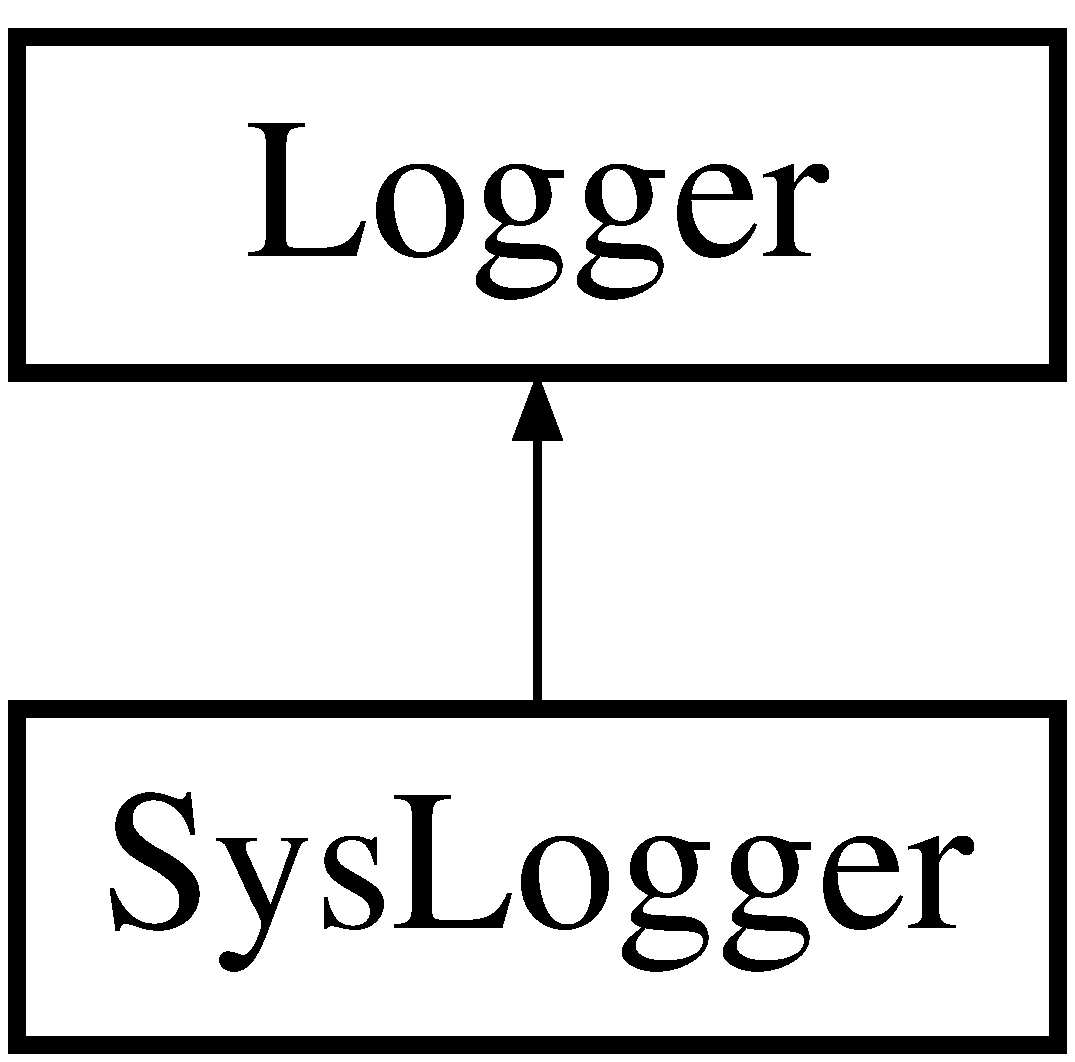
\includegraphics[height=2cm]{classSysLogger}
\end{center}
\end{figure}
\subsection*{Public Member Functions}
\begin{CompactItemize}
\item 
{\bf Sys\-Logger} (const char $\ast$ident=NULL, int option=LOG\_\-NDELAY, int facility=LOG\_\-USER, int n\-Log\-Level=ERROR\_\-MESSAGES\_\-LR)
\item 
virtual {\bf $\sim$Sys\-Logger} ()
\item 
virtual void {\bf log} (int level=ERROR\_\-MESSAGES\_\-LR, const string \&message=\char`\"{}\char`\"{}) const 
\end{CompactItemize}


\subsection{Detailed Description}
This {\bf Logger}{\rm (p.\,\pageref{classLogger})} provides an interface to the system logger.



\subsection{Constructor \& Destructor Documentation}
\index{SysLogger@{Sys\-Logger}!SysLogger@{SysLogger}}
\index{SysLogger@{SysLogger}!SysLogger@{Sys\-Logger}}
\subsubsection{\setlength{\rightskip}{0pt plus 5cm}Sys\-Logger::Sys\-Logger (const char $\ast$ {\em ident} = {\tt NULL}, int {\em option} = {\tt LOG\_\-NDELAY}, int {\em facility} = {\tt LOG\_\-USER}, int {\em n\-Log\-Level} = {\tt ERROR\_\-MESSAGES\_\-LR})\hspace{0.3cm}{\tt  [inline]}}\label{classSysLogger_a0}


Allows the user to tune the logger.\index{SysLogger@{Sys\-Logger}!~SysLogger@{$\sim$SysLogger}}
\index{~SysLogger@{$\sim$SysLogger}!SysLogger@{Sys\-Logger}}
\subsubsection{\setlength{\rightskip}{0pt plus 5cm}virtual Sys\-Logger::$\sim$Sys\-Logger ()\hspace{0.3cm}{\tt  [inline, virtual]}}\label{classSysLogger_a1}


Releases syslog connection.

\subsection{Member Function Documentation}
\index{SysLogger@{Sys\-Logger}!log@{log}}
\index{log@{log}!SysLogger@{Sys\-Logger}}
\subsubsection{\setlength{\rightskip}{0pt plus 5cm}void Sys\-Logger::log (int {\em level} = {\tt ERROR\_\-MESSAGES\_\-LR}, const string \& {\em message} = {\tt \char`\"{}\char`\"{}}) const\hspace{0.3cm}{\tt  [virtual]}}\label{classSysLogger_a2}


Handles receipt of preformatted messages.

Implements {\bf Logger} {\rm (p.\,\pageref{classLogger_a2})}.

The documentation for this class was generated from the following files:\begin{CompactItemize}
\item 
Sys\-Logger.hpp\item 
Sys\-Logger.cpp\end{CompactItemize}
